\chapter{Analyse et spécification des besoins}
\setlength{\intextsep}{6pt}
\setlength{\textfloatsep}{8pt}
\setlength{\floatsep}{6pt}
\setlength{\abovecaptionskip}{3pt}
\setlength{\belowcaptionskip}{1pt}
\setlength{\LTpre}{3pt}
\setlength{\LTpost}{3pt}

\newpage

%============================================================
\section{Introduction}
%============================================================

Le présent chapitre est dédié à la description des exigences fonctionnelles et non
fonctionnelles du logiciel de gestion des ressources humaines et de pointage automatique
par reconnaissance faciale. Ce chapitre contient l'information relative à l'environnement
logiciel, matériel et technologique requis pour le développement et l'utilisation du
logiciel proposé. Aussi, le chapitre contient la description de la méthodologie du travail
utilisée et basée sur la méthode Agile Scrum.

%============================================================
\section{Analyse des besoins}
%============================================================

Dans cette partie, nous détaillons les besoins du système, en identifiant les
fonctionnalités attendues ainsi que les contraintes techniques, sécuritaires et
ergonomiques associées.

\subsection{Besoins fonctionnels}

Les besoins fonctionnels du système de gestion RH et de pointage basé sur la reconnaissance
faciale correspondent aux différentes actions que chaque utilisateur doit pouvoir réaliser
pour que le système remplisse ses objectifs. Pour les formaliser, nous avons identifié les
acteurs et les cas d'utilisation du système conformément aux standards UML.

\subsubsection{Identification des acteurs}

L'analyse du système a permis de définir trois acteurs principaux :

\begin{itemize}
  \item \textbf{Employé :} Personne travaillant dans l'entreprise.
  \item \textbf{Responsable RH :} Membre du personnel ayant des droits spécifiques pour
        gérer les employés, les dossiers RH et générer des rapports.
  \item \textbf{Administrateur du logiciel :} Personne chargée de superviser la plateforme,
        de gérer les utilisateurs et leurs accès.
\end{itemize}

\subsubsection{Identification des cas d'utilisation}

Pour chaque acteur, les objectifs et fonctionnalités du système sont les suivants :

\paragraph{Fonctionnalités pour l'employé}

\begin{itemize}
  \item Enregistrer son visage : permettre à l'employé d'ajouter ses données faciales dans le système.
  \item Modifier ses informations personnelles : mettre à jour ses informations telles que l'adresse, le numéro de téléphone ou l'état civil.
  \item Consulter ses absences : visualiser son historique d'absences et de présences.
  \item Pointage faciale : effectuer l'enregistrement de présence à l'aide de la reconnaissance faciale.
  \item Consulter son salaire : accéder aux informations relatives à sa rémunération.
  \item Soumettre un  congé : soumettre une demande de congé au service concerné.
  \item Consulter historique : afficher les opérations et actions précédemment effectuées.
  \item Déposer un document : envoyer des fichiers ou justificatifs au système.
  
\end{itemize}

\paragraph{Fonctionnalités pour le responsable RH}

\begin{itemize}
  \item S'inscrire : permettre au responsable RH de créer un compte et d'accéder aux fonctionnalités dédiées.
  \item Visualiser le Dashboard RH : consulter les indicateurs clés, statistiques des employés et synthèses RH.
  \item Connexion de la plateforme aux caméras : configurer et gérer les flux vidéo pour la reconnaissance faciale.
  \item Gérer les comptes employés : ajouter, modifier, désactiver ou supprimer les profils des employés.
  \item Gérer les congés (validation / refus) : traiter les demandes de congé, les approuver ou les refuser et suivre leur historique.
  \item Gérer les salaires : consulter et mettre à jour les informations de paie et générer des fiches de salaire.
  \item Gérer les documents : superviser le dépôt, le classement et l'accès aux justificatifs et pièces administratives.
  \item Gérer historique et rapports : générer, consulter et exporter les rapports d'activité, d'absence et autres historiques.
\end{itemize}

\paragraph{Fonctionnalités pour l'administrateur}

\begin{itemize}
  \item Gérer les comptes des utilisateurs (responsable RH) du système : créer, modifier, désactiver ou supprimer les comptes des responsables RH afin de contrôler leur accès à la plateforme.
  \item Visualiser le Dashboard Administrateur : consulter les indicateurs globaux, les statistiques d'utilisation et les informations de supervision du système.
  
\end{itemize}

\subsubsection{Diagramme de cas d'utilisation global}

Toutes les fonctionnalités mentionnées précédemment pour les différents acteurs (Employé,
Responsable RH et Administrateur du logiciel) ont été regroupées dans un diagramme de cas
d'utilisation. Ce diagramme structuré permet de visualiser les interactions entre les
acteurs et le système. La figure~\ref{fig:usecase} présente ce diagramme de cas d'utilisation.

\begin{figure}[H]
  \centering
  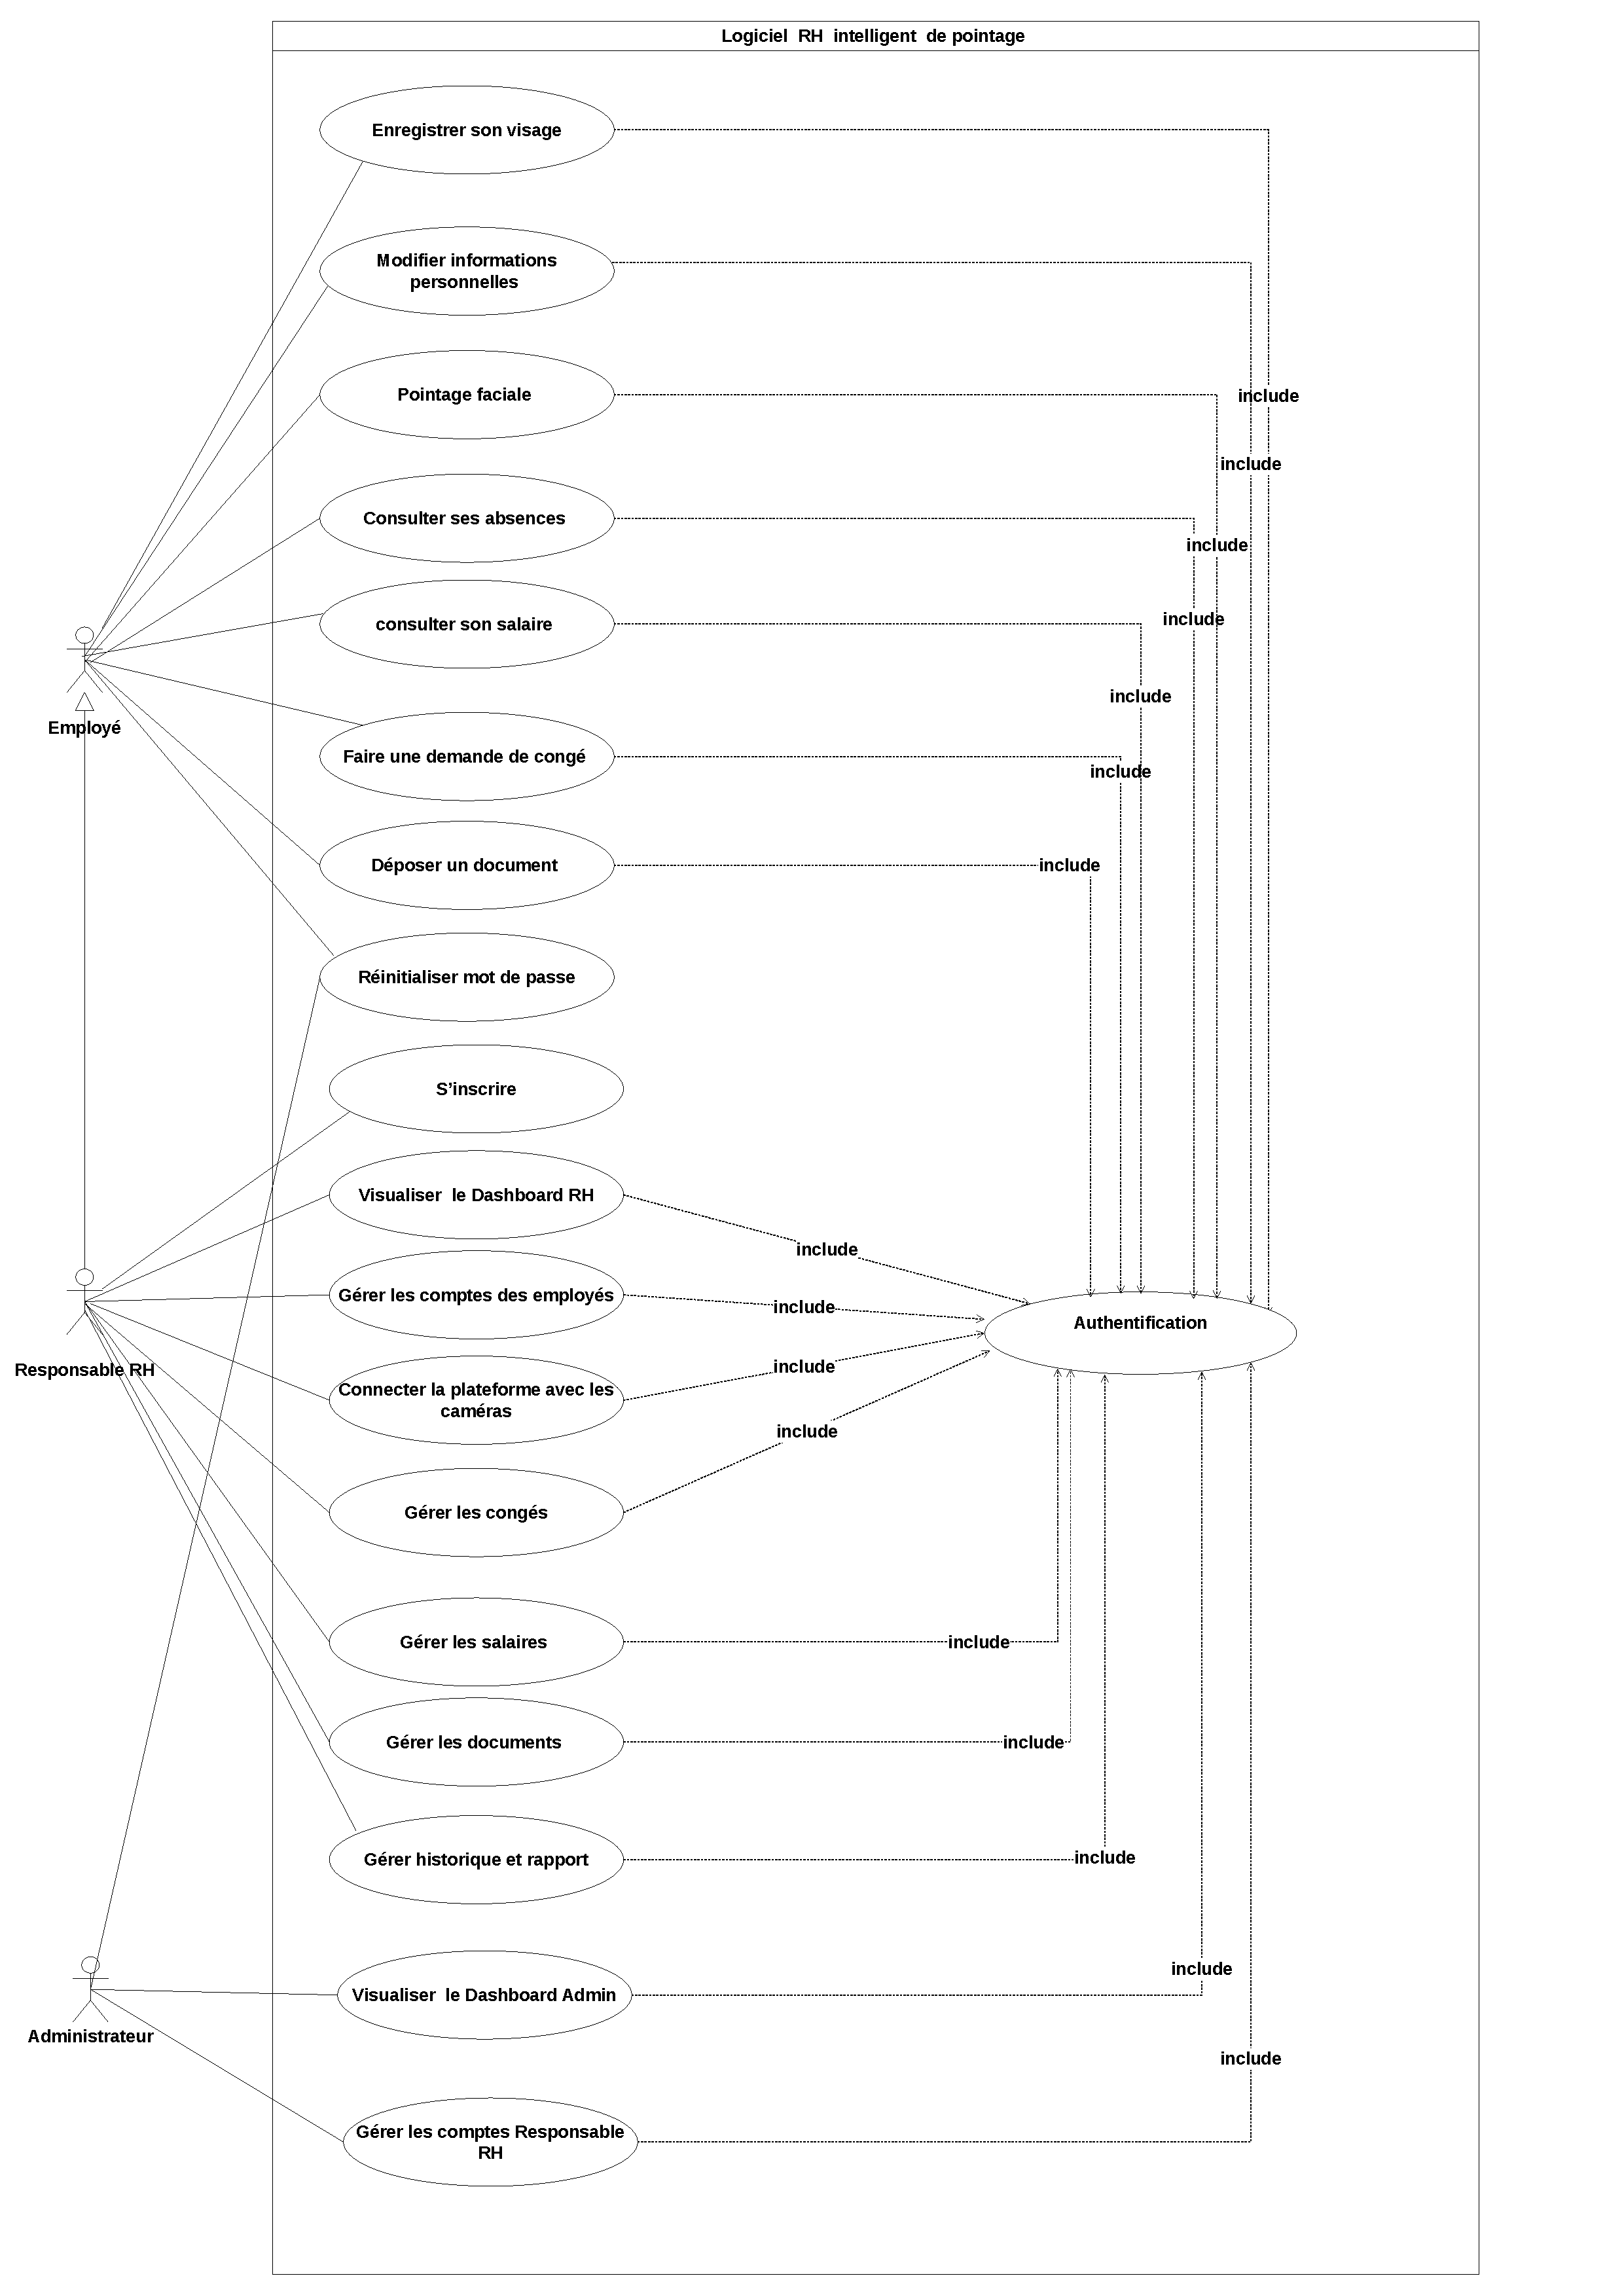
\includegraphics[
    width=0.8\paperwidth,
    height=1\textheight,
    keepaspectratio
  ]{projet/images/usecase/use.pdf}
  \caption{Diagramme de cas d'utilisation du système}
  \label{fig:usecase}
\end{figure}

\subsection{Besoins non fonctionnels}

Les besoins non fonctionnels définissent les contraintes et qualités attendues du système.

\begin{itemize}
  \item \textbf{Contraintes techniques :}
    \begin{itemize}
      \item Compatibilité avec les caméras standard.
      \item Temps de reconnaissance inférieur à 2 secondes.
      \item Base de données sécurisée et performante.
    \end{itemize}

  \item \textbf{Contraintes de sécurité :}
    \begin{itemize}
      \item Chiffrement des données sensibles.
      \item Authentification et autorisation des utilisateurs.
      
    \end{itemize}

  \item \textbf{Contraintes ergonomiques et esthétiques :}
    \begin{itemize}
      \item Interface intuitive et facile à utiliser.
      \item Navigation simple entre les fonctionnalités.
      \item Tableau de bord clair et lisible avec indicateurs visuels.
      \item Respect de l'identité visuelle de l'application et cohérence graphique.
    \end{itemize}
\end{itemize}

%============================================================
\section{Pilotage de projet avec Scrum}
%============================================================

Cette section présente l'application de la méthode Scrum dans le cadre du projet, en
détaillant l'organisation de l'équipe, la gestion du backlog ainsi que la planification
des différentes releases.

\subsection{Affectation des rôles Scrum}

L'équipe Scrum se compose de trois rôles différents, qui sont le Product Owner, le Scrum
Master et les développeurs. À chaque sprint, l'équipe Scrum est responsable de la création
d'un incrément de valeur à destination des utilisateurs et des clients.

Les rôles Scrum sont affectés comme suit :

\begin{itemize}
  \item \textbf{Product Owner :} BelHadj Mohamed
  \item \textbf{Scrum Master :} Amara Hiba
  \item \textbf{Développeurs :} Araar Mohamed et Mejri Louay
\end{itemize}

\subsection{Le Backlog de produit}

Le backlog du produit liste toutes les fonctionnalités, les exigences, les améliorations et
les correctifs à apporter à l'application à réaliser. Les différentes User Stories qui
composent le Backlog du produit représentent les objectifs à atteindre par l'équipe Scrum.
Le tableau~\ref{tab:backlog} illustre le backlog du produit du système à réaliser. Les
différentes user stories du backlog du produit sont ordonnées du plus prioritaires au moins
prioritaires. Les fonctionnalités prioritaires sont considérées comme indispensables pour le
système à mettre en œuvre, ces dernières permettant d'obtenir un produit qui contient le
minimum de fonctionnalités nécessaires pour être utilisé.

Une user story est souvent présentée de la manière suivante :
\og{}\textit{utilisateur + besoin + finalité}\fg{} avec

Le sprint backlog du projet et présenté par le tableau suivant :

\renewcommand{\arraystretch}{1.5}

\begin{longtable}{|>{\centering\arraybackslash}m{0.5cm}|
    >{\centering\arraybackslash}m{3cm}|
    >{\centering\arraybackslash}m{2.5cm}|
    >{\centering\arraybackslash}m{3cm}|
    >{\centering\arraybackslash}m{3cm}|
    >{\centering\arraybackslash}m{0.7cm}|
    >{\centering\arraybackslash}m{0.9cm}|}
\hline
\textbf{ID} & \textbf{User Story} & \textbf{En tant que} & \textbf{Je veux} &
\textbf{Afin de} & \textbf{P} & \textbf{C} \\
\hline
\endfirsthead
\hline
\textbf{ID} & \textbf{User Story} & \textbf{En tant que} & \textbf{Je veux} &
\textbf{Afin de} & \textbf{P} & \textbf{C} \\
\hline
\endhead

1  & Créer compte responsable RH    & Administrateur & créer un compte responsable RH    & administrer la plateforme        & 5 & 2 \\ \hline
2  & Modifier compte responsable RH & Administrateur & modifier un compte responsable RH & administrer la plateforme        & 4 & 2 \\ \hline
3  & Supprimer compte responsable RH& Administrateur & supprimer un compte responsable RH& administrer la plateforme        & 4 & 2 \\ \hline
4  & Visualiser le Dashboard Admin  & Administrateur & surveiller le fonctionnement global & assurer la stabilité du système & 5 & 4 \\ \hline
5  & S'inscrire                     & Responsable RH & créer mon compte sur la plateforme & accéder au système de gestion RH & 5 & 2 \\ \hline
6  & Visualiser le Dashboard RH     & Responsable RH & visualiser les indicateurs RH globaux & piloter l'activité RH         & 5 & 3 \\ \hline
7  & Créer compte employé           & Responsable RH & créer un compte employé           & permettre l'accès au système     & 5 & 2 \\ \hline
8  & Modifier compte employé        & Responsable RH & modifier un compte employé        & mettre à jour les informations et les accès de l'employé & 4 & 2 \\ \hline
9  & Supprimer compte employé       & Responsable RH & supprimer un compte employé       & désactiver définitivement l'accès de l'employé au système & 4 & 2 \\ \hline
10 & Connecter la plateforme aux caméras & Responsable RH & configurer et connecter les caméras & activer le pointage automatique & 5 & 5 \\ \hline
11 & Valider congé                  & Responsable RH & valider une demande de congé      & autoriser l'absence              & 5 & 2 \\ \hline
12 & Refuser congé                  & Responsable RH & refuser une demande de congé      & gérer les absences               & 5 & 2 \\ \hline
13 & Attribuer prime                & Responsable RH & attribuer une prime à un employé  & récompenser les employés         & 3 & 2 \\ \hline
14 & Attribuer déduction            & Responsable RH & appliquer une déduction à un employé & gérer la paie avec précision  & 4 & 3 \\ \hline
15 & Mettre à jour statut salaire   & Responsable RH & mettre à jour le statut du salaire & assurer la paie                 & 5 & 3 \\ \hline
16 & Consulter documents            & Responsable RH & consulter les documents envoyés   & vérifier les pièces              & 3 & 2 \\ \hline
17 & Valider document               & Responsable RH & approuver un document             & contrôler les absences           & 4 & 2 \\ \hline
18 & Rejeter document               & Responsable RH & refuser un document               & contrôler les absences           & 4 & 2 \\ \hline
19 & Modifier salaire               & Responsable RH & ajouter un salaire à un employé   & assurer une gestion correcte de la paie & 3 & 3 \\ \hline
20 & Générer rapport               & Responsable RH & générer un rapport                & exploiter les données RH         & 3 & 3 \\ \hline
21 & Consulter historique        & Responsable RH & consulter l'historique des actions effectuées & assurer le suivi et la traçabilité des opérations RH & 4 & 3 \\ \hline

22 & Enregistrer le visage          & Employé        & enregistrer mon visage            & permettre le pointage automatique & 5 & 5 \\ \hline
23 & Modifier infos personnelles    & Employé        & modifier mes informations personnelles & maintenir mes données à jour & 3 & 2 \\ \hline
24 & Consulter ses absences         & Employé        & consulter mes absences            & suivre ma présence               & 3 & 2 \\ \hline
25 & Consulter ses primes           & Employé        & consulter mes primes              & connaître mes avantages          & 2 & 1 \\ \hline
26 & Consulter déduction            & Employé        & voir mes déductions               & comprendre ma fiche de paie      & 2 & 1 \\ \hline
27 & Consulter son salaire          & Employé        & voir le statut de mon salaire     & savoir s'il est versé            & 3 & 1 \\ \hline
28 & Soumettre un congé             & Employé        & envoyer une demande de congé      & obtenir une autorisation d'absence & 5 & 2 \\ \hline
29 & Déposer un document            & Employé        & déposer un document               & justifier une absence            & 4 & 3 \\ \hline
30 & Pointage faciale               & Employé        & pointer ma présence par reconnaissance faciale & automatiser le pointage et éviter les oublis de pointage & 5 & 5 \\ \hline
31 & S'authentifier                 & Employé + Responsable RH + Administrateur & me connecter et me déconnecter    & accéder à mon espace sécurisé    & 5 & 2 \\ \hline

\caption{Backlog de produit}
\label{tab:backlog}
\end{longtable}

\subsection{Planification de releases}

À partir du product backlog défini en amont, le travail a été organisé selon une approche agile basée sur des cycles courts et itératifs. Chaque user story a été priorisée en fonction de sa valeur métier et de ses dépendances techniques, afin de déterminer un ordre d’exécution cohérent et optimal. En prenant en compte la taille de l’équipe ainsi qu’un calendrier global de quatre mois, la planification a été structurée en quatre sprints , couvrant la période du 14 février 2026 au 29 mai 2026. Les fonctionnalités essentielles, notamment la gestion des accès, l’administration des comptes et le pointage intelligent par reconnaissance faciale, ont été planifiées en priorité afin de garantir des fondations techniques robustes dès les premières itérations. L’ensemble des sprints est organisé en deux releases complémentaires, permettant une livraison progressive et maîtrisée du système.

\subsubsection*{Release 1 : Fondations \& Présence Intelligente}

La première release, du 14/02/2026 au 06/04/2026, regroupe les deux premiers sprints et constitue la base fonctionnelle du système. Elle couvre la gestion des accès, l’authentification sécurisée, l’administration des comptes ainsi que la mise en place du pointage intelligent par reconnaissance faciale. Cette phase permet de stabiliser l’architecture et de valider les fonctionnalités essentielles.
La répartition des user stories est détaillée dans le tableau suivant :
\begin{longtable}{|c|>{\raggedright\arraybackslash}p{4.2cm}|
    >{\centering\arraybackslash}p{2.5cm}|
    >{\centering\arraybackslash}p{3.5cm}|
    >{\raggedright\arraybackslash}p{5.5cm}|}
\hline
\textbf{ID} & \textbf{Nom Sprint} & \textbf{Story ID} & \textbf{Durée} & \textbf{Objectif} \\
\hline
\endfirsthead
\hline
\textbf{ID} & \textbf{Nom Sprint} & \textbf{Story ID} & \textbf{Durée} & \textbf{Objectif} \\
\hline
\endhead
1 & Gestion des Accès et Administration des Comptes
  & 1-2-3-5-7-8-9-31
  & 14/02/2026 -- 11/03/2026
  & Mettre en place l'authentification du système, la gestion des comptes
    (Administrateur, Responsable RH et Employé), la réinitialisation du mot de
    passe ainsi que le contrôle d'accès sécurisé à la plateforme. \\ \hline
2 & Pointage Intelligent et Suivi de Présence
  & 10-22-23-24-30
  & 12/03/2026 -- 06/04/2026
  & Implémenter le pointage automatique par reconnaissance faciale, connecter
    les caméras et permettre le suivi des présences, absences et informations
    personnelles des employés. \\ \hline
\caption{Release 1}
\end{longtable}

\subsubsection*{Release 2 : Gestion RH Complète et Pilotage}
La deuxième release, du 07/04/2026 au 29/05/2026, regroupe les sprints suivants et introduit les fonctionnalités avancées. Elle inclut la gestion des congés, des documents administratifs et de la paie, ainsi que les modules de reporting, de traçabilité et de pilotage RH via tableaux de bord. Cette phase finalise le système en enrichissant ses capacités fonctionnelles et décisionnelles.
La répartition des user stories est détaillée dans le tableau suivant :
\begin{longtable}{|c|>{\raggedright\arraybackslash}p{4.2cm}|
    >{\centering\arraybackslash}p{2.5cm}|
    >{\centering\arraybackslash}p{3.5cm}|
    >{\raggedright\arraybackslash}p{5.5cm}|}
\hline
\textbf{ID} & \textbf{Nom Sprint} & \textbf{Story ID} & \textbf{Durée} & \textbf{Objectif} \\
\hline
\endfirsthead

3 & Gestion  des Congés et des Documents Administratifs
  & 11-12-13-14-15-16-17-18-19-25-26-27-28-29
  & 07/04/2026 -- 02/05/2026
  & Développer les fonctionnalités liées à la gestion des congés, documents,
    primes, déductions et salaires, ainsi que la validation, le rejet et le
    dépôt des documents administratifs. \\ \hline
4 & Pilotage RH, Reporting et Traçabilité
  & 4-6-20-21
  & 03/05/2026 -- 29/05/2026
  & Implémenter les tableaux de bord (Administrateur et Responsable RH),
    la génération des rapports, la consultation de l'historique des actions
    RH. \\ \hline
\caption{Release 2}
\end{longtable}

\subsection{Diagramme de Gantt}

Ce diagramme montre la planification temporelle du projet en illustrant l'organisation des
sprints, des tâches et des différentes phases de développement du système RH intelligent.

\begin{figure}[H]
  \centering
  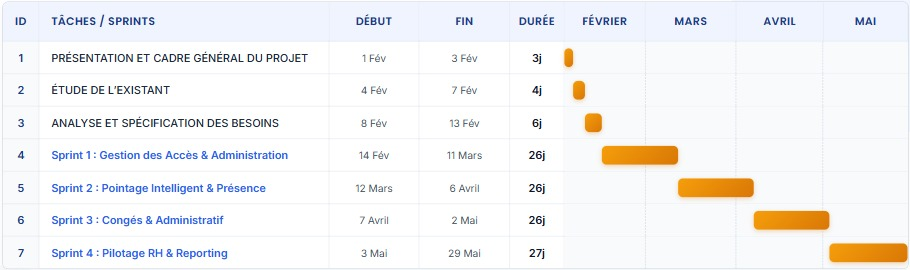
\includegraphics[width=\textwidth]{projet/images/daigramme_de_gant.jpeg}
  \caption{Diagramme de Gantt du projet}
  \label{fig:gantt}
\end{figure}

%============================================================
\section{Étude technique}
%============================================================

Cette étude technique a pour but d'analyser en détail les différentes composantes et
mécanismes impliqués dans notre logiciel.

\subsection{Environnement matériel}

La réalisation de notre projet utilise deux machines de caractéristiques différentes :

\begin{table}[H]
\centering
\renewcommand{\arraystretch}{1.5}
\begin{tabular}{|p{5cm}|p{8cm}|}
\hline
\textbf{Marque}              & Dell Latitude 5530 \\ \hline
\textbf{Mémoire}             & 24,0 Go \\ \hline
\textbf{Processeur}          & 12th Gen Intel(R) Core(TM) i5-1245U (1.60 GHz) \\ \hline
\textbf{Disque dur}          & 725 Go \\ \hline
\textbf{Système d'exploitation} & Windows 11 Professionnel \\ \hline
\end{tabular}
\caption{Environnement matériel 1}
\end{table}

\begin{table}[H]
\centering
\renewcommand{\arraystretch}{1.5}
\begin{tabular}{|p{5cm}|p{8cm}|}
\hline
\textbf{Marque}              & Dell vostro 3530  \\ \hline
\textbf{Mémoire}             & 16,0 Go \\ \hline
\textbf{Processeur}          & AMD Ryzen 7 5700U with Radeon Graphics \\ \hline
\textbf{Disque dur}          & 1 To \\ \hline
\textbf{Système d'exploitation} & Windows 11 Professionnel \\ \hline
\end{tabular}
\caption{Environnement matériel 2}
\end{table}

\subsection{Environnement logiciel}

Dans cette partie, nous détaillons l'ensemble des environnements logiciels utilisés dans
le cadre du projet, incluant les outils de conception, de développement, ainsi que les
langages, frameworks et bibliothèques employés.

\subsubsection{Logiciels de conception}

Lors de la conception de notre site, nous avons utilisé les logiciels suivants :

\begin{table}[H]
\centering
\renewcommand{\arraystretch}{1.5}
\begin{tabular}{|m{3cm}|m{10cm}|}
\hline
\centering
\vspace{0.2cm}

\includegraphics[height=2cm]{projet/images/Figma-logo.png}
&
\textbf{Figma :} Figma est un outil de conception d'interfaces graphiques permettant de
créer, partager et tester des designs pour les sites web, les applications mobiles et
d'autres produits numériques. Il facilite également la collaboration en temps réel entre
les membres d'une équipe.\cite{figma}
\\ \hline
\centering
\vspace{0.2cm}

\includegraphics[height=2cm]{projet/images/ps adobe.png}
&
\textbf{Adobe Photoshop :} Adobe Photoshop est un logiciel de retouche et de traitement
d'images numériques. Il permet la modification, la création et l'amélioration des images
et des supports graphiques professionnels.\cite{photoshop}
\\ \hline
\centering
\vspace{0.2cm}

\includegraphics[height=2cm]{projet/images/draw io.png}
&
\textbf{draw.io :} draw.io est un outil de création de diagrammes en ligne permettant de
réaliser des organigrammes, des diagrammes UML, des schémas réseau et d'autres
représentations graphiques de manière simple et efficace.\cite{drawio}
\\ \hline

\centering
\vspace{0.2cm}

\includegraphics[height=2cm]{projet/images/overlef.png}
&
\textbf{Overleaf :}  outil de rédaction de documents scientifiques en LaTeX
en ligne, utilisé pour la rédaction et la mise en forme du rapport de
stage.\cite{overleaf}
\\ \hline

\end{tabular}
\caption{Environnement logiciel de conception}
\end{table}

\subsubsection{Logiciels de développement}

Lors du développement de notre site, nous avons utilisé les logiciels suivants :

\begin{table}[H]
\centering
\renewcommand{\arraystretch}{1.4}
\begin{tabular}{|m{3cm}|m{10cm}|}
\hline
\centering
\vspace{0.2cm}
\includegraphics[height=2cm]{projet/images/vs.jpeg}
&
\textbf{Visual Studio Code :} VSCode est un éditeur de code source et un IDE open-source
compatible avec Windows, Linux et Mac.\cite{Visual Studio Code}
\\ \hline
\centering
\vspace{0.2cm}
\includegraphics[height=2cm]{projet/images/tt.jpeg}
&
\textbf{GitHub :} GitHub est un service cloud qui nous aide à stocker et gérer le code,
à suivre et contrôler les modifications.\cite{GitHub}
\\ \hline
\centering
\vspace{0.2cm}
\includegraphics[height=2cm]{projet/images/postamn.jpeg}
&
\textbf{Postman :} Postman est un outil de développement et de test d'API qui permet
d'envoyer des requêtes HTTP (GET, POST, PUT, DELETE…), d'analyser les réponses du
serveur et de vérifier le bon fonctionnement des services web.\cite{Postman}
\\ \hline
\end{tabular}
\caption{Environnement logiciel de développement}
\end{table}

\subsubsection{Langages de développement}

Lors du développement de notre site, nous avons utilisé les langages suivants :

\renewcommand{\arraystretch}{1.4}
\setlength{\LTleft}{\fill}
\setlength{\LTright}{\fill}
\begin{longtable}{|m{14cm}|}
\hline
\textbf{HTML :} HTML (HyperText Markup Language) est le langage de base du Web qui
structure le contenu des pages.\cite{HTML} \\ \hline
\textbf{CSS :} CSS (Cascading Style Sheets) permet de définir la présentation visuelle
des pages web.\cite{CSS} \\ \hline
\textbf{JavaScript :} JavaScript (JS) est un langage de programmation léger interprété
(ou compilé juste-à-temps) avec des fonctions de première classe. Bien qu'il soit le
langage de script le plus connu pour les pages Web, il est utilisé pour les interactions
dynamiques et les animations.\cite{JavaScript} \\ \hline
\textbf{TypeScript :} Extension de JavaScript utilisée pour améliorer la fiabilité et
la maintenance du code.\cite{TypeScript} \\ \hline
\textbf{Python :} Langage utilisé pour développer le modèle de reconnaissance faciale
et le serveur backend.\cite{Python} \\ \hline
\textbf{SQL :} Langage utilisé pour gérer la base de données.\cite{SQL} \\ \hline
\caption{Langages de développement}
\end{longtable}

\subsubsection{Frameworks et bibliothèques}

Lors du développement de notre site, nous avons utilisé les frameworks et bibliothèques
suivants :

\begin{longtable}{|m{14cm}|}
\hline
\textbf{Next.js :} Framework React full-stack permettant de développer le frontend et
le backend dans une seule application.\cite{Next.js} \\ \hline
\textbf{React :} Bibliothèque JavaScript utilisée pour construire l'interface
utilisateur.\cite{React} \\ \hline
\textbf{Flask :} Micro-framework pour développer des applications web et des
API.\cite{Flask} \\ \hline
\textbf{OpenCV :} Bibliothèque de vision par ordinateur pour le traitement
d'images.\cite{OpenCV} \\ \hline
\textbf{MediaPipe :} Bibliothèque utilisée pour la détection des visages et des points
caractéristiques.\cite{MediaPipe} \\ \hline
\textbf{TensorFlow :} Bibliothèque d'apprentissage automatique utilisée pour
l'entraînement du modèle.\cite{TensorFlow} \\ \hline
\caption{Frameworks et bibliothèques}
\end{longtable}

%============================================================
\section{Architecture de la solution}
%============================================================

Dans cette section, nous présentons l'architecture logique et logicielle de notre système.

\subsection{Architecture logique}

L'architecture logique identifie les composants logiciels nécessaires à l'implémentation
d'une solution et décrit les relations existant entre ces composants. Notre logiciel RH
intelligent repose sur une architecture en trois tiers (\textit{3-tier architecture}),
permettant une séparation claire des responsabilités. Elle se compose d'une couche
présentation responsable de l'interface utilisateur, d'une couche métier contenant les
règles de gestion, et d'une couche d'accès aux données assurant la persistance des
informations. Cette structuration améliore la maintenabilité, la modularité et
l'évolutivité du système.

\begin{figure}[H]
  \centering
  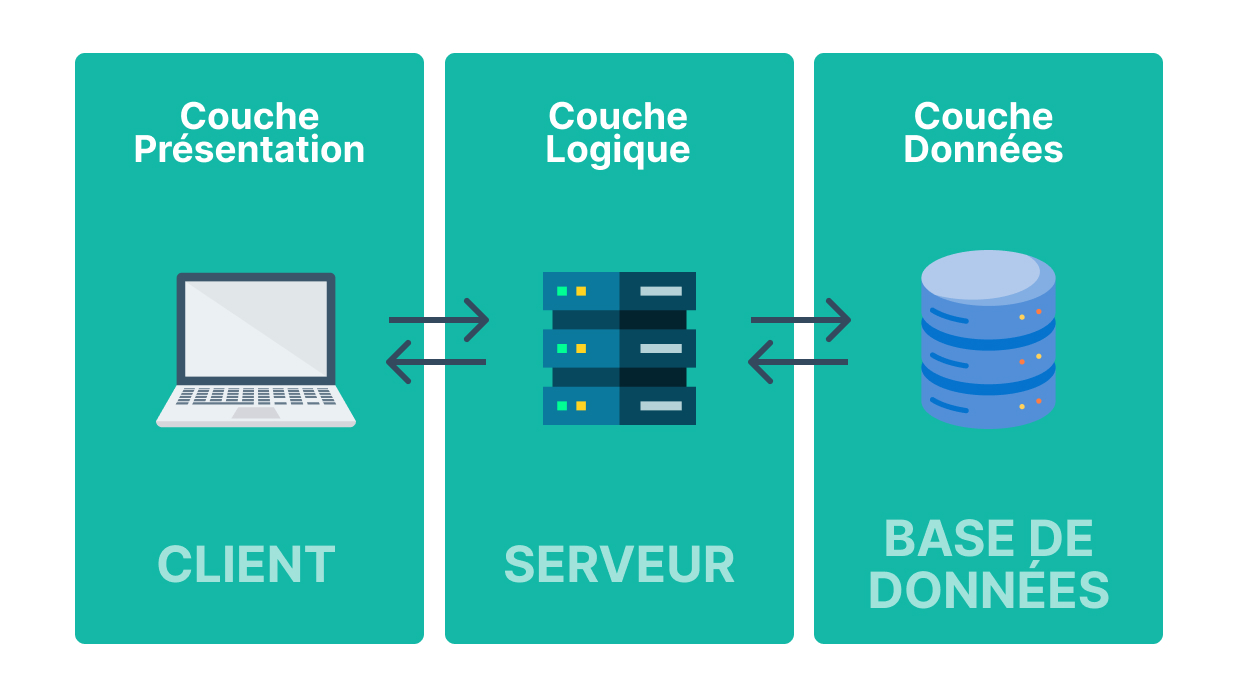
\includegraphics[scale=0.2]{projet/images/architecture logique.jpg}
  \caption{Architecture logique}
\end{figure}

\subsection{Architecture logicielle}

Le système adopte une \textbf{architecture logicielle découplée orientée API}, dans
laquelle chaque couche est développée de manière indépendante et communique avec les
autres exclusivement via des \textbf{interfaces REST}. Cette approche s'inscrit dans une
\textbf{architecture 3 tiers} en précisant l'organisation interne de chaque couche.

La \textbf{couche présentation} est assurée par \textbf{Next.js}, un framework React
qui offre un rendu hybride combinant le \textbf{rendu côté serveur (SSR)} et le
\textbf{rendu côté client (CSR)}, garantissant ainsi de bonnes performances et une
expérience utilisateur fluide. Elle communique avec le backend à travers des
\textbf{requêtes HTTP sécurisées} et adapte dynamiquement l'interface en fonction du
rôle de l'utilisateur.

La \textbf{couche métier} repose sur \textbf{Flask}, un framework Python léger et
flexible, permettant de développer des \textbf{API REST} de manière simple et efficace.
L'organisation du code est structurée de manière à assurer une \textbf{séparation claire
des responsabilités} et à faciliter la maintenance du système.

Le système intègre également un \textbf{module d'intelligence artificielle} dédié à la
\textbf{reconnaissance faciale}. Ce module est développé en \textbf{Python} et intégré
au backend Flask sous forme de \textbf{services spécialisés}. Il permet d'automatiser
certaines tâches comme le \textbf{pointage} ou la \textbf{vérification d'identité},
tout en restant \textbf{indépendant et évolutif}.

Enfin, la \textbf{couche de données} est assurée par \textbf{MySQL}, un système de
gestion de base de données relationnelle permettant de stocker et de gérer efficacement
les informations liées aux employés, aux congés et aux différentes opérations du système.

\begin{figure}[H]
  \makebox[\textwidth][l]{%
    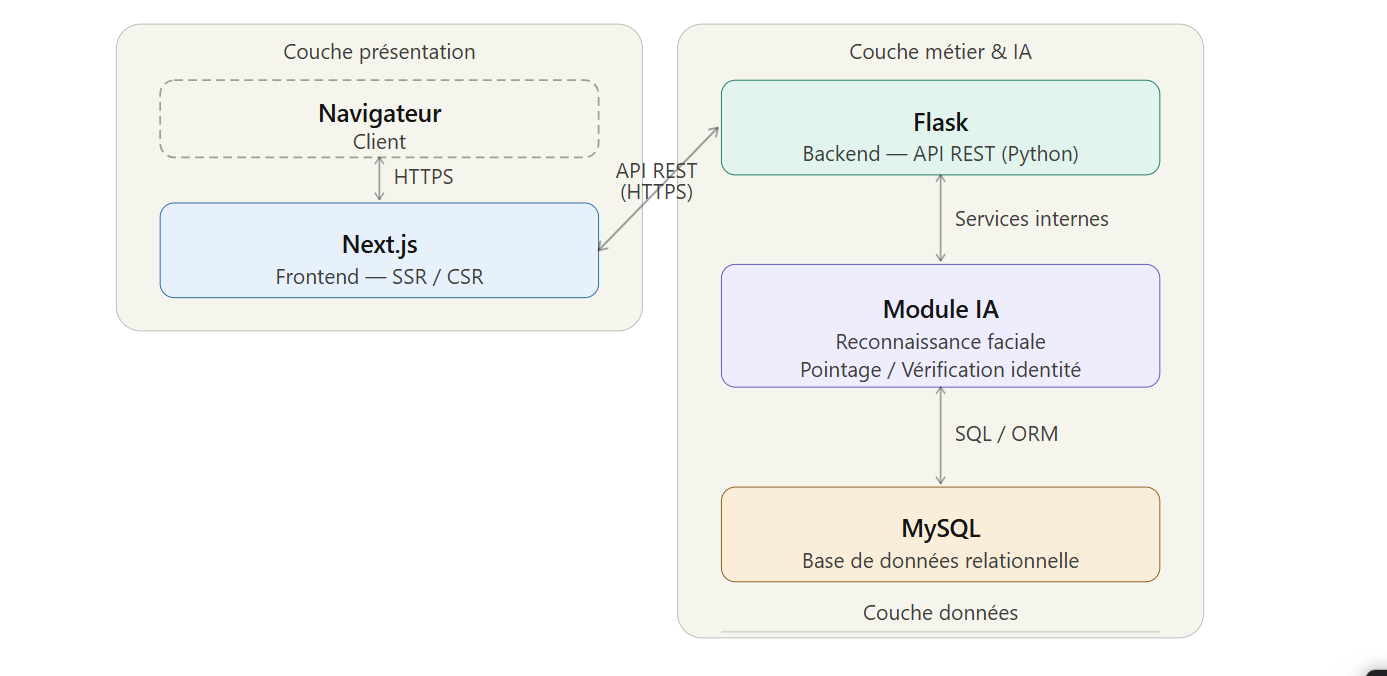
\includegraphics[width=0.9\textwidth]{projet/images/xc.png}
  }
  \caption{Architecture logicielle du système}
\end{figure}

%============================================================
\section{Conclusion}
%============================================================

Dans ce chapitre, nous avons abordé de manière détaillée les besoins fonctionnels et non
fonctionnels du projet, présenté l'environnement logiciel nécessaire à sa réalisation,
ainsi que les différents rôles Scrum impliqués. De plus, nous avons élaboré le product
backlog avec une répartition en releases. En conclusion, ce chapitre a posé les bases
essentielles pour la gestion efficace du projet. Le prochain chapitre se concentrera sur
le contenu spécifique de la première release, mettant en lumière les fonctionnalités clés
à développer pour répondre aux besoins identifiés.